%
%  CSE 150. Assignment 1
%
%  Created by Pierre Louis Gottfrois on 2012-01-18.
%  Copyright (c) 2012. All rights reserved.
%
\documentclass[]{article}

% Use utf-8 encoding for foreign characters
\usepackage[utf8]{inputenc}
\usepackage{color}

% Setup for fullpage use
\usepackage{fullpage}

% More symbols
\usepackage{amsmath}
\usepackage{amssymb}

% Surround parts of graphics with box
\usepackage{boxedminipage}

% Package for including code in the document
\usepackage{listings}

% If you want to generate a toc for each chapter (use with book)
\usepackage{minitoc}

% This is now the recommended way for checking for PDFLaTeX:
\usepackage{ifpdf}

\ifpdf
\usepackage[pdftex]{graphicx}
\else
\usepackage{graphicx}
\fi
\usepackage{tikz,tkz-tab}

\title{CSE 150. Assignment 1}
\author{Pierre-Louis Gottfrois}

\date{2012-01-18}

\begin{document}

\ifpdf
\DeclareGraphicsExtensions{.pdf, .jpg, .tif}
\else
\DeclareGraphicsExtensions{.eps, .jpg}
\fi

\maketitle

\section{Kullback-Leibler distance}

\begin{center}
  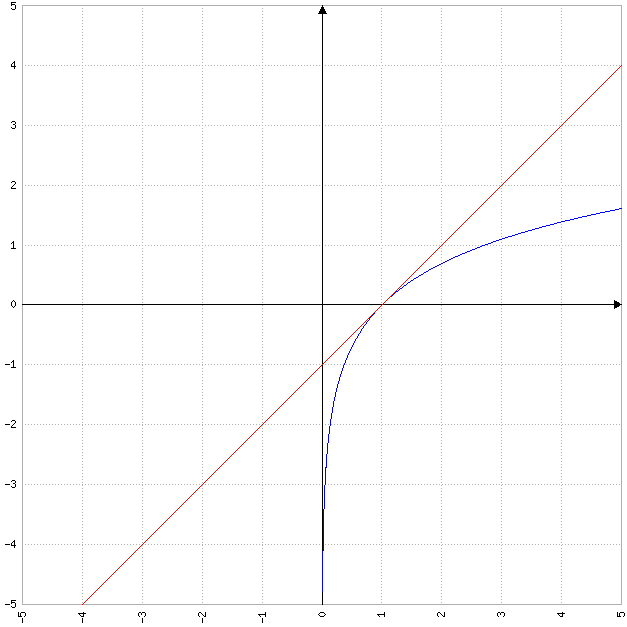
\includegraphics[scale=0.7]{hw1.png}
\end{center}

\newpage

\begin{enumerate}
  \item We can see with this graph that the function than \textcolor{blue}{$log(x)$} $<=$ \textcolor{red}{$x-1$}.

  Differentiation of $log(x)-(x-1)$ : \\

  $f(x) = log(x) - (x - 1)$ \\
  \\
  $f'(x) = 1/x*ln(e) - (1 - 0)$ \\
  $f'(x) = (1/x)-1$ \\

  \begin{center}
    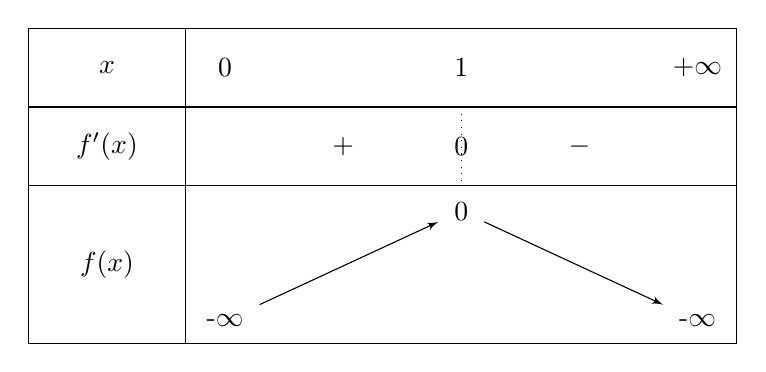
\begin{tikzpicture}
    \tkzTabInit{$x$/1,$f'(x)$/1,$f(x)$/2}{$0$,$1$,$+\infty$}
    \tkzTabLine{,+,z,-}
    \tkzTabVar{-/-$\infty$,+/$0$,-/-$\infty$}
    \end{tikzpicture}
  \end{center}

  We then can conclude that $log(x) <= x-1$

  \item If $p_{i} = q_{i}$ then :

  $KL(p,p) = \sum_{i} p_{i}log(p_{i}/p_{i})$ \\
  $KL(p,p) = \sum_{i} p_{i}log(1)$ \\
  $KL(p,p) = \sum_{i} p_{i}*0$ \\
  $KL(p,p) = 0$


  Then $KL(p,q) >= 0$ if $p_{i} = q_{i}$

  \item
\end{enumerate}

\newpage

\section{Conditional independence}

Let : \\

$P(X,Y|Z) = \frac{P(X,Y,Z)}{P(Z)}$ \\

$P(X,Y|Z) = \frac{P(X,Y,Z)}{P(Y,Z)} * \frac{P(Y,Z)}{P(Z)}$ \\

$P(X,Y|Z) = P(X|Y,Z) * \frac{P(Y,Z)}{P(Z)}$ \\

$P(X,Y|Z) = P(X|Y,Z) * P(Y,Z)$ \\

As $P(X|Y,Z) = P(X|Z)$ then : \\

$P(X,Y|Z) = P(X|Z) * P(Y,Z)$ \\

The three statements are equivalent.

\newpage

\section{Creative writing}

\begin{enumerate}
  \item Lets choose the random variables as follow : \\

  X = Burglary ? \\
  Y = Yann calls ? \\
  Z = Alarm ? \\

  So that \\
  $P(X =1|Y =1) > P(X =1),$ \\
  $P(X =1|Y =1, Z =1) < P(X =1|Y =1)$

  \item Lets choose the random variables as follow : \\

  X = Alarm ? \\
  Y = Yann calls ? \\
  Z = Zoe calls ? \\

  So that \\
  $P(X =1) < P(X =1|Y =1) < P(X =1|Y =1, Z =1)$

  \item Lets choose the random variables as follow : \\

  X = Alarm ? \\
  Y = Earthquake ? \\
  Z = Zoe calls ? \\

  So that \\
  $P(X =1, Y =1) = P(X =1)P(Y =1)$ \\
  $P(X =1, Y =1|Z =1) = P(X =1|Z =1)P(Y =1|Z =1)$
\end{enumerate}

\newpage

\section{Probabilistic inference}

\begin{flushleft}
  Conditional independence assumptions : \\

  $P(B|E) = P(B)$ \\
  $P(J|A) = P(J|A,B,E)$ \\
  $P(M|A) = P(M|A,B,E,J)$
\end{flushleft}

a)
\begin{align*}
  P(B=1|M=1) & = \frac{P(M=1|B=1)P(B=1)}{P(M=1)} \\
  \\
  P(M=1) & = \sum_{a,b,e,j} P(M=1,A=a,B=b,E=e,J=j) \\
  &= \sum_{a} P(M=1,A=a) \\
  &= \sum_{a} P(M=1|A=a)P(A=a) \\
  &= P(M=1|A=0)P(A=0) + P(M=1|A=1)P(A=1) \\
  &= 0,01*P(A=0) + 0,70*P(A=1) \\
  \\
  P(A=1) & = \sum_{b,e} P(E=e,B=b,A=1) \\
  &= \sum_{b,e} P(E=e)P(B=b|E=e)P(A=1|E=e,B=b) \\
  &= \sum_{b,e} P(E=e)P(B=b)P(A=1|E=e,B=b) \\
  &= P(E=0)P(B=0|E=0)P(A=1|E=0,B=0) + P(E=1)P(B=0|E=1)P(A=1|E=1,B=0) + \\
  & P(E=0)P(B=1|E=0)P(A=1|E=0,B=1) + P(E=1)P(B=1|E=1)P(A=1|E=1,B=1) \\
  &= (1-0,002)(1-0,001)(0,001) + (0,002)(1-0,001)(0,29) + \\
  & (1-0,002)(0,001)(0,94) + (0,002)(0,001)(0,95) \\
  &= 0,00252\\
  \\
  P(M=1) & = 0,01*P(A=0) + 0,70*P(A=1) \\
  &= 0,01*(1-0,00252) + 0,70*0,00252 \\
  &= 0,01174
\end{align*}

\begin{align*}
  P(M=1|B=1) & = \sum_{a} P(M=1,A=a|B=1) \\
  &= \sum_{a} P(M=1|A=a,B=1)P(A=a|B=1) \\
  &= \sum_{a} P(M=1|A=a)P(A=a|B=1) \\
  \\
  P(A=1|B=1) & = \sum_{e} P(A=1,E=e|B=1) \\
  &= \sum_{e} P(A=1|E=e,B=1)P(E=e,B=1) \\
  &= \sum_{e} P(A=1|E=e,B=1)P(E=e) \\
  &= P(A=1|E=0,B=1)P(E=0) + P(A=1|E=1,B=1)P(E=1) \\
  &= (0,94)(1-0,002) + (0,95)(0,002) \\
  &= 0,94002 \\
  \\
  P(M=1|B=1) & = \sum_{a} P(M=1|A=a)P(A=a|B=1) \\
  &= P(M=1|A=0)P(A=0|B=1) + P(M=1|A=1)P(A=1|B=1) \\
  &= (0,01)(1-0,94002) + (0,70)(0,94002) \\
  &= 0,65861 \\
  \\
  P(B=1|M=1) & = \frac{P(M=1|B=1)P(B=1)}{P(M=1)} \\
  &= \frac{0,65861*0,001}{0,01174} \\
  &= 0,0561
\end{align*}

b)
\begin{align*}
  P(B=1|M=1,E=1) & = \frac{P(M=1|B=1,E=1)P(B=1|E=1)}{P(M=1|E=1)} \\
  &= \frac{P(M=1|B=1,E=1)P(B=1)}{P(M=1|E=1)} \\
  \\
  P(M=1|E=1) & = \sum_{a} P(M=1,A=a|E=1) \\
  &= \sum_{a} P(M=1|A=a|E=1)P(A=a|E=1) \\
  &= \sum_{a} P(M=1|A=a|E=1)P(A=a) \\
  &= P(M=1|A=0)P(A=0) + P(M=1|A=1)P(A=1) \\
  &= (0,01)(1-0,00252) + (0,70)(0,00252) \\
  &= 0,01174 \\
  \\
  P(M=1|B=1,E=1) & = P(M=1|B=1) \\
  &= 0,65861 \\
  \\
  P(B=1|M=1,E=1) & = \frac{P(M=1|B=1,E=1)P(B=1)}{P(M=1|E=1)} \\
  &= \frac{0,65861*0,001}{0,01174} \\
  &= 0,0561 \\
  \\
  P(B=1|M=1) = P(B=1|M=1,E=1)
\end{align*}

c)
\begin{align*}
  P(A=1|J=0) & = \frac{P(J=0|A=1)P(A=1)}{P(J=0)} \\
  \\
  P(J=0) & = \sum_{a} P(J=0,A=a) \\
  &= \sum_{a} P(J=0|A=a)P(A=a) \\
  &= P(J=0|A=0)P(A=0) + P(J=0|A=1)P(A=1) \\
  &= (1-0,05)(1-0,00252) + (1-0,90)(0,00252) \\
  &= 0,94786 \\
  \\
  P(A=1|J=0) & = \frac{P(J=0|A=1)P(A=1)}{P(J=0)} \\
  &= \frac{(1-0,90)(0,00252)}{0,94786} \\
  &= 0,00027 \\
\end{align*}

d)
\begin{align*}
  P(A=1|J=0,M=1) & = \frac{P(J=0,M=1|A=1)P(A=1)}{P(J=0,M=1)} \\
  &= \frac{P(J=0|A=1)P(M=1|A=1,J=0)P(A=1)}{P(J=0,M=1)} \\
  &= \frac{P(J=0|A=1)P(M=1|A=1)P(A=1)}{P(J=0,M=1)} \\
  &= \frac{(1-0,90)(0,70)(0,00252)}{P(J=0,M=1)} \\
  \\
  P(J=0,M=1) & = \sum_{a} P(A=a,J=0,M=1) \\
  &= \sum_{a} P(A=a)P(J=0|A=a)P(M=1|A=a,J=0) \\
  &= \sum_{a} P(A=a)P(J=0|A=a)P(M=1|A=a) \\
  &= P(A=0)P(J=0|A=0)P(M=1|A=0) + \\
  & P(A=1)P(J=0|A=1)P(M=1|A=1) \\
  &= (1-0,00252)(1-0,05)(0,01) + (0,00252)(1-0,90)(0,70) \\
  &= 0,00964 \\
  \\
  P(A=1|J=0,M=1) & = \frac{(1-0,90)(0,70)(0,00252)}{P(J=0,M=1)} \\
  &= \frac{(1-0,90)(0,70)(0,00252)}{0,00964} \\
  &= 0,0183 \\
  \\
  P(A=1|J=0) > P(A=1|J=0,M=1) \\
\end{align*}

e)
\begin{align*}
  P(A=1|B=0) & = \sum_{e} P(A=1,E=e|B=0) \\
  &= \sum_{e} P(A=1|E=e,B=0)P(E=e,B=0) \\
  &= \sum_{e} P(A=1|E=e,B=0)P(E=e) \\
  &= P(A=1|E=0,B=0)P(E=0) + P(A=1|E=1,B=0)P(E=1) \\
  &= (0,001)(1-0,002) + (0,29)(0,002) \\
  &= 0,001578 \\
\end{align*}

f)
\begin{align*}
  P(A=1|B=0,M=1) & = \frac{P(M=1|A=1,B=0)P(A=1|B=0)}{P(M=1|B=0)} \\
  \\
  P(M=1|B=0) & = \sum_{a} P(M=1,A=a|B=0) \\
  &= \sum_{a} P(A=a|B=0)P(M=1|A=a,B=0) \\
  &= P(A=0|B=0)P(M=1|A=0,B=0) + \\
  & P(A=1|B=0)P(M=1|A=1,B=0) \\
  &= P(A=0|B=0)(0,01) + (0,001578)(0,70) \\
  \\
  P(A=0|B=0) & = \sum_{e} P(A=0,E=e|B=0) \\
  &= \sum_{e} P(A=0|E=e,B=0)P(E=e,B=0) \\
  &= \sum_{e} P(A=0|E=e,B=0)P(E=e) \\
  &= P(A=0|E=0,B=0)P(E=0) + P(A=0|E=1,B=0)P(E=1) \\
  &= (1-0,001)(1-0,002) + (1-0,29)(0,002) \\
  &= 0,998422 \\
  \\
  P(M=1|B=0) & = P(A=0|B=0)(0,01) + (0,001578)(0,70) \\
  &= (0,998422)(0,01) + (0,001578)(0,70) \\
  &= 0,01109 \\
  \\
  P(A=1|B=0,M=1) & = \frac{P(M=1|A=1,B=0)P(A=1|B=0)}{P(M=1|B=0)} \\
  &= \frac{0,70*0,001578}{0,01109} \\
  &= 0,09960 \\
  \\
  P(A=1|B=0,M=1) > P(A=1|B=0)\\
\end{align*}

All the results above seems consistent with commonsense patterns or reasoning. \\

\end{document}
